\let\negmedspace\undefined
\let\negthickspace\undefined
\documentclass[journal]{IEEEtran}
\usepackage[a5paper, margin=10mm, onecolumn]{geometry}
%\usepackage{lmodern} % Ensure lmodern is loaded for pdflatex
\usepackage{tfrupee} % Include tfrupee package

\setlength{\headheight}{1cm} % Set the height of the header box
\setlength{\headsep}{0mm}     % Set the distance between the header box and the top of the text
\usepackage{gvv-book}
\usepackage{gvv}
\usepackage{cite}
\usepackage{amsmath,amssymb,amsfonts,amsthm}
\usepackage{algorithmic}
\usepackage{graphicx}
\usepackage{textcomp}
\usepackage{xcolor}
\usepackage{txfonts}
\usepackage{listings}
\usepackage{enumitem}
\usepackage{mathtools}
\usepackage{gensymb}
\usepackage{comment}
\usepackage[breaklinks=true]{hyperref}
\usepackage{tkz-euclide} 
\usepackage{listings}
% \usepackage{gvv}                                        
\def\inputGnumericTable{}                                 
\usepackage[latin1]{inputenc}                                
\usepackage{color}                                            
\usepackage{array}                                            
\usepackage{longtable}                                       
\usepackage{calc}                                             
\usepackage{multirow}                                         
\usepackage{hhline}                                           
\usepackage{ifthen}                                           
\usepackage{lscape}



\usepackage{amsmath,amssymb}
\usepackage{booktabs}
\usepackage{tikz}
\usetikzlibrary{arrows.meta,angles,quotes}

\begin{document}

\bibliographystyle{IEEEtran}
\vspace{3cm}

\title{1.9.3}
\author{EE25BTECH11014 - Bhoomika Lokesh}
% \maketitle
% \newpage
% \bigskip
{\let\newpage\relax\maketitle}

\renewcommand{\thefigure}{\theenumi}
\renewcommand{\thetable}{\theenumi}
\setlength{\intextsep}{10pt} % Space between text and floats


\numberwithin{equation}{enumi}
\numberwithin{figure}{enumi}
\renewcommand{\thetable}{\theenumi}

\textbf{Question:}   \textit{AOBC} is a rectangle whose three vertices are $\brak{0,-3}$ $\brak{0,0}$ $\brak{4,0}$.The length of its diagonal is\rule{2cm}{0.4pt}.

\textbf{Solution:}  Given the points $\vec{A},\vec{O}$ and $\vec{B}:$\\
\begin{table}[H]    
  \centering
  \begin{tabular}{|c|c|c|c|}
\hline
Angle (\(\alpha\)) & \(\cos(\alpha)\) & Value & Axis \\
\hline
\(90^\circ\) & \(\cos(90^\circ) = 0\) & \(l = 0\) & x-axis \\
\(60^\circ\) & \(\cos(60^\circ) = \frac{1}{2}\) & \(m = \frac{1}{2}\) & y-axis \\
\(30^\circ\) & \(\cos(30^\circ) = \frac{\sqrt{3}}{2}\) & \(n = \frac{\sqrt{3}}{2}\) & z-axis \\
\hline
\end{tabular}
  \caption{Vectors of the points}
  \label{tab:1.9.3}
\end{table}

\end{frame}

Determining the Coordinates of Point \vec{C}:
\begin{align}
 \vec{A} = \myvec {4\\0 }
 \vec{B} = \myvec {0\\-3}
\end{align}

 Since $\vec{C}$ is opposite to $\vec{O}$ in the rectangle,
 
 \begin{align}
\vec{C} = \vec{A} + \vec{B}=\myvec{4\\0}+ \myvec{0\\-3}=\myvec{4\\-3}
 \end{align}
\begin{align}
\therefore \vec{C}=\myvec{4\\-3}
\end{align}

We know that the length of the diagonal vector is magnitude of the vector $\vec{C}$.\\

\begin{align}
\vec{C}= \myvec{4 \\ -3} 
\end{align}

\begin{align}
\left|\vec{C} \right| &= \sqrt{ \vec{C}^T \cdot \vec{C}}
 \end{align}
 \begin{align}
     \vec{C}^T= \myvec{4 & -3} 
 \end{align}    
\begin{align}
      \vec{C}^T \cdot \vec{C}=\myvec{4 & -3}\myvec{4 \\ -3} = 4^2 + (-3)^2 = 16 + 9 = 25
\end{align}
\begin{align}  
      \left|\vec{C}\right| &= \sqrt{25} = 5 
 \end{align}
 \begin{center}
Therefore the lenght of the diagonal is $5$.
 \end{center}

See Fig 0.1,
\begin{figure}[H]
\begin{center}
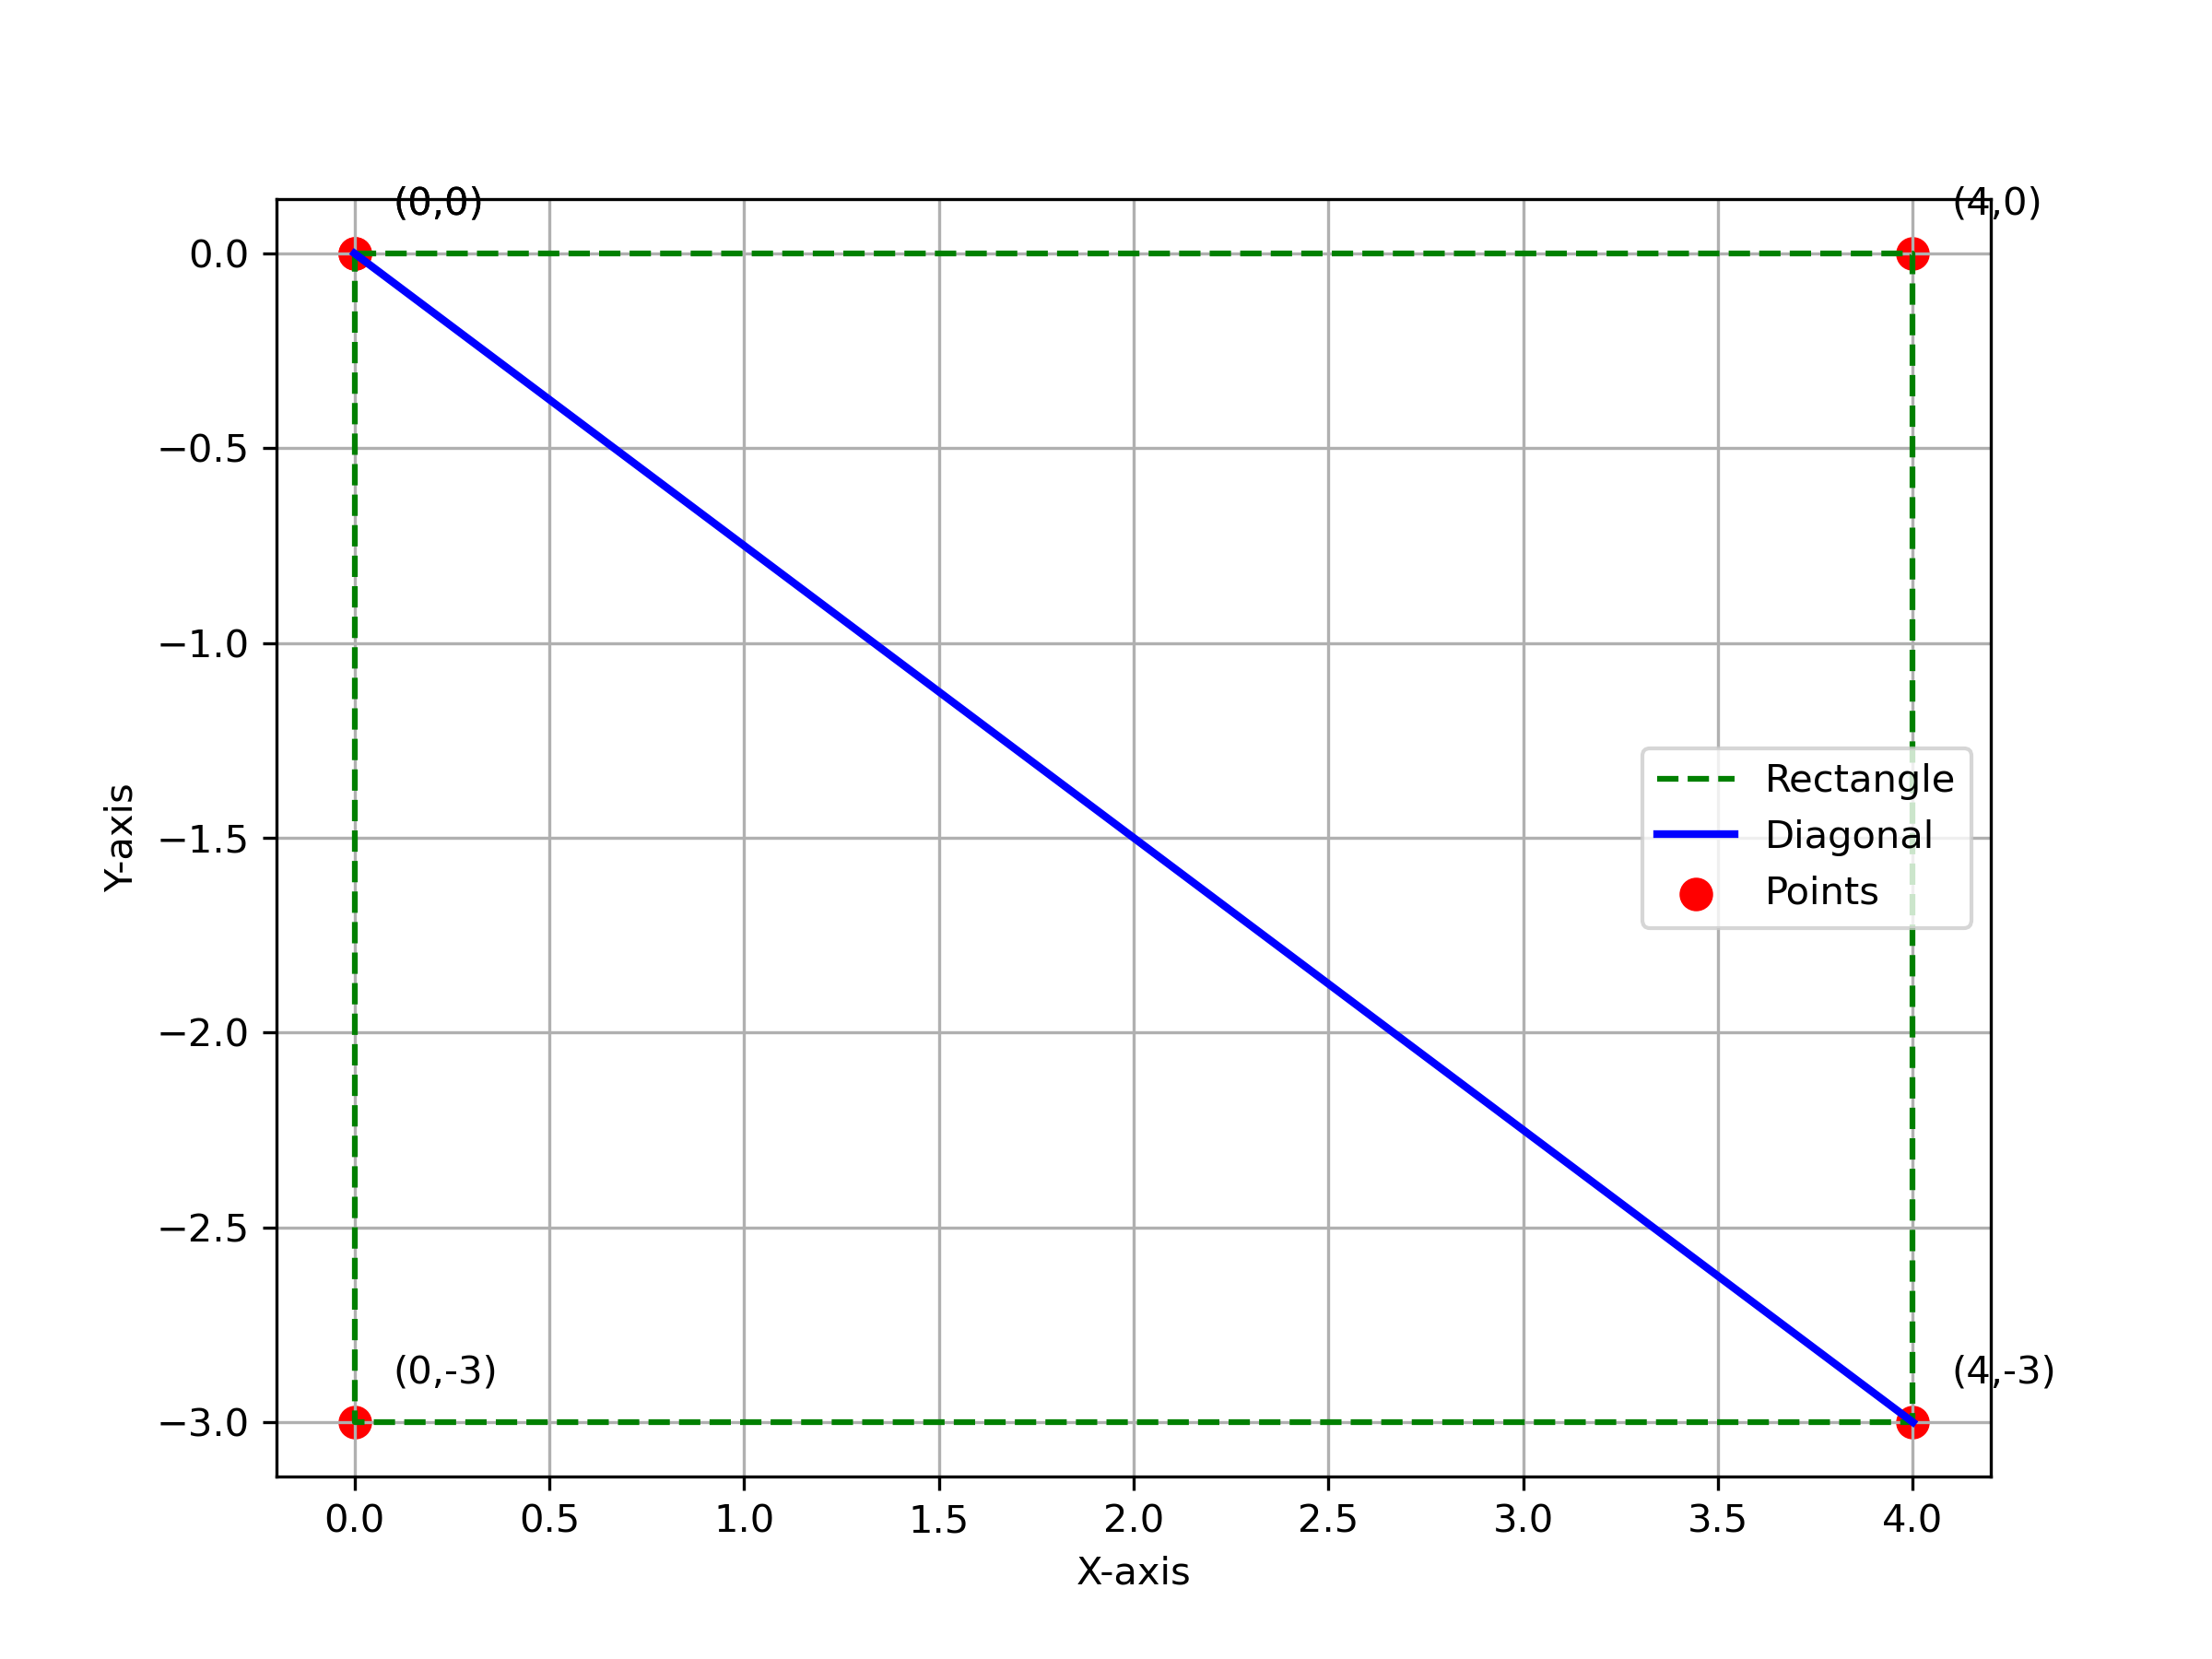
\includegraphics[width=0.7\columnwidth]{Figs/fig2.png}
\end{center}
\caption{Graph}
\label{fig:fig.py}
\end{figure}

 
\end{document}